\documentclass[
	ngerman,
	ruledheaders=section,
	class=report,
	thesis={type=Dokumentation},
	ignore-missing-data=true,
	accentcolor=9c,
	custommargins=false,
	marginpar=false,
	parskip=half-,
	fontsize=11pt,
]{tudapub}

% compatibility with older pdflatex versions
\usepackage{iftex}
\ifPDFTeX
	\usepackage[utf8]{inputenc}
\fi

% language packages
\usepackage[english, main=ngerman]{babel}
\usepackage[autostyle]{csquotes}

% tables
\usepackage{tabularx}
\usepackage{booktabs}

% mathematics
\usepackage{mathtools}
\usepackage{amssymb}
\usepackage{siunitx}
\sisetup{locale=DE}

% further packages
\usepackage[skip=10pt]{caption}
\usepackage{graphics,graphicx}
\usepackage[sf, SF]{subfigure}
\usepackage{listings}
\lstset{numbers=left, 
		numberstyle=\tiny, 
		numbersep=10pt, 
		frame=tlbr,
		framesep=5pt,
		backgroundcolor=\color{lightgray}, 
		xleftmargin=25pt, 
		xrightmargin=5pt, 
		showstringspaces=false, 
		tabsize=4}
\usepackage{epstopdf}
\usepackage{float}

% custom commands
\let\file\texttt
\let\code\texttt
\let\tbs\textbackslash
\let\pck\textsf
\let\cls\textsf
\newcommand{\mr}[1]{\mathrm{#1}}
\def\code#1{\begin{small}\texttt{#1}\end{small}}

% start document
\setlength\intextsep{22pt}
\begin{document}

\Metadata{
	title=1. Hausübung - OpenCL,
	author=Leon Bohmann, Jonathan Stollberg
}

\title{1. Hausübung - OpenCL}
\author[]{Leon Bohmann (2493657) und Jonathan Stollberg (247775)}
\submissiondate{\today}

\maketitle
\tableofcontents

\chapter{Einführung}
In dieser Hausübung ging es darum die Berechnung eines Matrix-Vektor-Produkts gemäß
\begin{align*}
	c_{i} = A_{ij}b_{j}
\end{align*}
in der Programmiersprache \textit{Java} zu implementieren. Dabei soll die Matrix $\mathbf{A}$ stets quadratisch sein, d.h. $\mathbf{A} \in \mathbb{R}^{m\times m}$ und $\mathbf{b} \in \mathbb{R}^{m}$. Die Implementierung wurde sequentiell und parallel umgesetzt, wobei darauf geachtet wurde, dass das Programm sowohl auf der CPU mittels Streams als auch auf der GPU mittels der Schnittstelle \textit{OpenCL} parallelisiert ist.

Das Programm kann über die Kommandozeile mit zwei optionalen (und untrennbaren) Argumenten aufgerufen werden. Das erste Argument repräsentiert dabei die Problemgröße $m$, das zweite Argument legt die \textit{local size} fest, die der \textit{OpenCL}-Kernel anfragt. Wird das Programm ganz ohne Argumente aufgerufen, so wird die Berechnung für verschiedene vordefinierte $m$ und \textit{local sizes} ausgeführt:
\begin{lstlisting}[language=bash]
$ java -jar HighPerformanceSimulation.jar
$ java -jar HighPerformanceSimulation.jar 1000 10
\end{lstlisting}

Im Folgenden sollen nun kurz wichtige Aspekte der Implementierung erläutert und anschließend die Performance der sequentiellen und parallelen Berechnungen für verschiedene $m$ analysiert und beurteilt werden.

\chapter{Sequentieller Algorithmus}
Zu Beginn des Programmaufrufs wird ausgehend von $m$ eine Zufallsmatrix $\mathbf{A}$ sowie ein Zufallsvektor $\mathbf{b}$ generiert. Diese werden als eindimensionale short-Arrays gespeichert, sodass auf das Element $A_{ij}$ über Index $i\times m + j$ zugegriffen wird. Für $\mathbf{b}$ ist der Zugriff über Indizes trivial.

Nachdem das Ergebnis-Array $\mathbf{c}$ der Länge $m$ initialisiert wurde, lässt sich die sequentielle Matrix-Vektor-Multiplikation nun mit wenigen Zeilen Code analog zur Einstein'schen Summenkonvention mithilfe von for-Schleifen implementieren:
\begin{lstlisting}[language=java]
short[] c = new short[m];
for (int i = 0; i < m; i++) {
	for (int j = 0; j < m; j++) {
		c[i] += A[i * m + j] * b[j];
	}
}
\end{lstlisting}
Selbstverständlich muss der Code noch in eine Klassenstruktur bzw. eine Methode eingebunden werden. Für Weitere Details zur Implementierung wird an dieser Stelle an den beiliegenden Code in der Datei \textit{MatrixVector.java} verwiesen.

\chapter{Paralleler Algorithmus mittels OpenCL}

Zur Implementierung mit \textit{OpenCL }waren einige Schritte zur Initialisierung nötig. Die Verwendete \textit{Java OpenCL} Library (\textit{JOCL}) ist ein Low-Level-API Wrapper. Es waren also mehrere aufwendige OpenCL-Calls nötig, um die gewünschte Funktionalität zu erreichen. Die Implementierung des Kernels erfolgte in einer \textit{C99}-Notation, welche für den \textit{OpenCL} Compiler vorgegeben war.

\section{Funktion des Kernels}
Folgend ist der Source-Code des Kernels dargestellt:
\begin{lstlisting}[language=c,label=kernel_source]
__kernel void matrix_vec(
	__global const short *lhs, 
	__global const short *rhs, 
	__global short *result, 
	const int d) {
		int gid = get_global_id(0);
		result[gid] = 0;		
		for(int i = 0; i < d; ++i) {
			result[gid] += lhs[gid * size + i] * rhs[i];
		}
};
\end{lstlisting}
Mit der Instruktion \code{\_\_kernel} wird dem \textit{OPCL} Compiler mitgeteilt, dass es sich um einen Einstiegspunkt handelt. Mit \code{\_\_global} markierte Argumente sind Strukturen aus dem globalen Speicher, welcher von allen Kernels angesprochen werden kann. Bei dem letzten Argument handelt es sich um die Gesamt-Größe der übergebenen (1D-)Arrays, da der Kernel keine andere Möglichkeit hat die übergebenen Matrix-Größen zu erfahren (die Pointer \code{*lhs}, \code{*rhs} und \code{*result} zeigen nur auf den Anfang der entsprechenden Arrays).

Jedes Work-Item (1 Work-Item = 1 Kernel-Ausführung) erhält vom Host (\textit{JOCL}) eine eindeutige ID. Diese erhält man mit \code{get\_global\_id}. Das Argument \code{0} definiert dabei die x-Richtung, da globale IDs auch mehrdimensional aufgereiht sein können. Mithilfe dieser ID wird eine Matrix-Zeile mit der Right-Hand-Side (\code{rhs}, dem Vektor) multipliziert. Das Ergebnis wird an der entsprechenden Stelle im Ergebnis-Array gespeichert. Mit anderen Worten: Die Matrix-Vektor-Multiplikation wird Zeilenweise in Kernels übergeben.

\section{Ablauf der Initialisierung}
Der Ablauf der Initialisierung verläuft wie folgt:
\begin{enumerate}
	\item Erhalte Anzahl an Plattformen
	\item Erhalte spezifische Plattform-IDs
	\item Verwende 1. gefundene Plattform
	\item Erhalte Anzahl an Devices auf Plattform
	\item Verwende 1. gefundenes Device
	\item Context für das Device erstellen
	\item CommandQueue für das Device erstellen	
\end{enumerate}

\subsection*{Context und CommandQueue}
Mit dem so generierten Context und der CommandQueue können dann jegliche weiteren Befehle ausgeführt werden. Der Context liefert dabei nötige infrastrukturelle Methoden und die CommandQueue dient der Kommunikation mit dem zugrundeliegenden Device. Im Regelfall sollten diese Objekte nach ihrer Verwendung verworfen und so für die Garbage Collection (GC) freigegeben werden. In diesem Fall wird die Referenz auf diese Objekte in der Klasse \code{OpenCL} gespeichert, um bei mehrfachem Aufruf erneute Instanzierungen zu vermeiden.

\subsection*{Kernel-Kompilierung}
Um Code an die Grafik-Karte oder andere Compute Units (CU) zu übergeben, bedarf es noch weiterer Arbeit. Zunächst muss ein sogenanntes Programm erzeugt werden (\code{clCreateProgramWithSource}). Dazu verwendet man einen in \textit{C99} verfassten Sourcecode, welcher durch \textit{OpenCL} unterhalb von \textit{JOCL} kompiliert wird (\code{clBuildProgram}). Das ausführbare Programm muss dann noch in einen Kernel überführt werden (\code{clCreateKernel}). Der Kernel wird letztlich von \textit{JOCL} auf die CU übertragen und kann dann ausgeführt werden. Wie die Referenzen aus dem vorigen Absatz wird auch der Kernel nicht verworfen.

\subsection*{Speicher}
Da sich Grafikkarte und CPU keinen Speicher teilen, müssen sogenannte Buffer implementiert werden, die Speicherzugriffe zwischen den beiden dedizierten Speichern koordinieren. Für weitere Details zur Implementierung wird an die Datei \textit{MatrixVector.java} bzw. die Methode \code{MatrixVector.initParallel(long lws, int availableUnits)} verwiesen.

Um die zugrundeliegende Struktur in den globalen Speicher der Grafikkarte zu kopieren, werden Buffer erstellt, die den Inhalt des Host-Speichers (für den CPU verfügbarer Speicher) kopieren.

\subsection*{Kernel-Argumente}
Um dem Host mitzuteilen, welche Argumente an die Kernel übergeben werden sollen, müssen diese noch mit \code{clSetKernelArg(...)} definiert werden. Hier ist darauf zu achten, dass die korrekten Objekt-Typen angegeben werden, da es sonst zu Memory-Leaks oder Schreiben in geschütztem Speicher kommt.

\subsection*{Starten der Kernel}
Hat man die Initialisierung abgeschlossen, folgt das Starten der Kernels. Dazu wird eine globale und eine lokale Work-Size definiert. \textit{Global} bedeutet hierbei den vollständigen Umfang der Work-Items (in diesem Fall die Menge an Zeilen in der Matrix) und \textit{lokal} die Anzahl an gleichzeitig ausgeführten Work-Items (Kernel) innerhalb einer Work-Group. Aufgrund der Architektur von Grafikkarten (zumindest von NVIDIA) ist es ratsam, die Local-Work-Size(LWS) entsprechend der sogenannten Warp-Size zu definieren. Während Work-Groups auf sogenannten Threads ausgeführt werden, werden die beinhalteten Work-Items dann nochmal auf einzelne CU verteilt. Die Anzahl der so verteilten Work-Items nennt man Warp-Size. Bei häuslichen Tests auf einer \textit{GTX 1060} mit einer Warp-Size von 32 erhält man eine LWS von ebenjenen 32. Bei kleineren LWS als 32 bleiben Rechenkapazitäten der GPU unbenutzt.

Die Kernels werden zuletzt mit \code{clEnqueueNDRangeKernel} an die CommandQueue übergeben. Hierbei werden die globalen und lokalen Arbeitsgrößen übergeben und der Host übernimmt die Verteilung.

Das übergeben der Kernels an die CommandQueue garantiert noch nicht, dass diese auch ausgeführt werden. Da der Host durch die übergebenen Kernel-Argumente weiß, welches Argument die Ausgabe des Kernels ist, kann er mit der Ausführung der Kernels warten, bis dieser angefordert wird.

\subsection*{Kernel-Ergebnisse auslesen}
Ähnlich wie das kopieren vom Host-Speicher in den Ziel-Speicher müssen beim Lesen der Ergebnisse die Arrays vom Ziel-Speicher zurück in den Host-Speicher geladen werden. Dies geschieht mit \code{clEnqueueReadBuffer}.

Durch das Anfordern des Ergebnis-Speichers werden die zuvor eingereihten Kernels ausgeführt. Dieses Verhalten ist zur Messung nicht vorteilhaft, da auch das Auslesen des Speichers eine gewisse Zeit in Anspruch nehmen kann. Die Ausführung der Kernels wird daher nach \code{clEnqueueNDRangeKernel} mit Aufruf von \code{clFinish(OpenCL.commandQueue)} forciert (siehe \code{MatrixVector.parallel(..)}).

\chapter{Performance-Analyse}
Die Performance-Tests wurden auf dem Lichtenberg-Hochleistungsrechner der Technischen Universität Darmstadt durchgeführt. Zu diesem Zwecke wurde ein SLURM-Skript geschrieben, welches einen Rechenknoten mit einer GPU des Typs \textit{NVIDIA A100-PCIE-40GB} sowie 30 GB Speicher pro CPU anfordert. Damit wurden die Tests für $m \in \{10, 1000, 2000, 4000, 8000, 10000, 15000\}$ gerechnet. Die \code{local\_work\_size} wurde dabei zunächst von \textit{OpenCL} selbst festgelegt, anschließend aber auch noch variiert. Um die Rechenzeit möglichst unverfälscht zu zu untersuchen, wurde der Warmup der \textit{OpenCL}-Parallelisierung in allen Messungen ignoriert. Außerdem wurden folgende Hardwarespezifikationen von \textit{OpenCL} ausgelesen:
\begin{itemize}
	\item \code{CL\_DEVICE\_MAX\_WORK\_GROUP\_SIZE} = 262144
	\item \code{CL\_DEVICE\_MAX\_WORK\_ITEM\_DIMENSIONS} = 3
	\item \code{CL\_DEVICE\_MAX\_WORK\_ITEM\_SIZES} = 1024, 1024, 64
	\item \code{CL\_DEVICE\_MAX\_COMPUTE\_UNITS} = 108
\end{itemize}

\begin{figure}[h!tb]
	\centering
	\subfigure[Rechenzeit.]{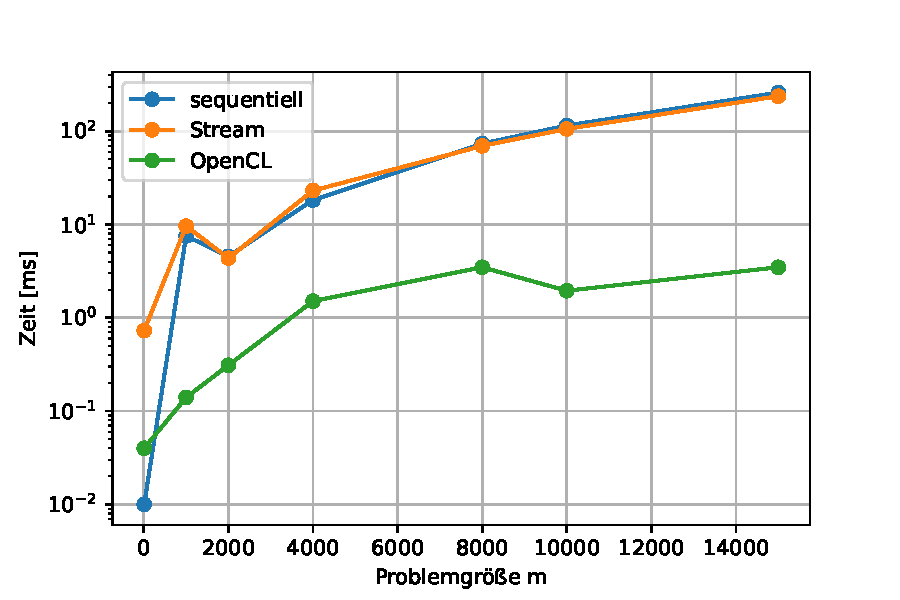
\includegraphics[width=9.2cm]{auto_lws.pdf}}\hspace{-0.8cm}
	\subfigure[Speedup durch die GPU-Parallelisierung.]{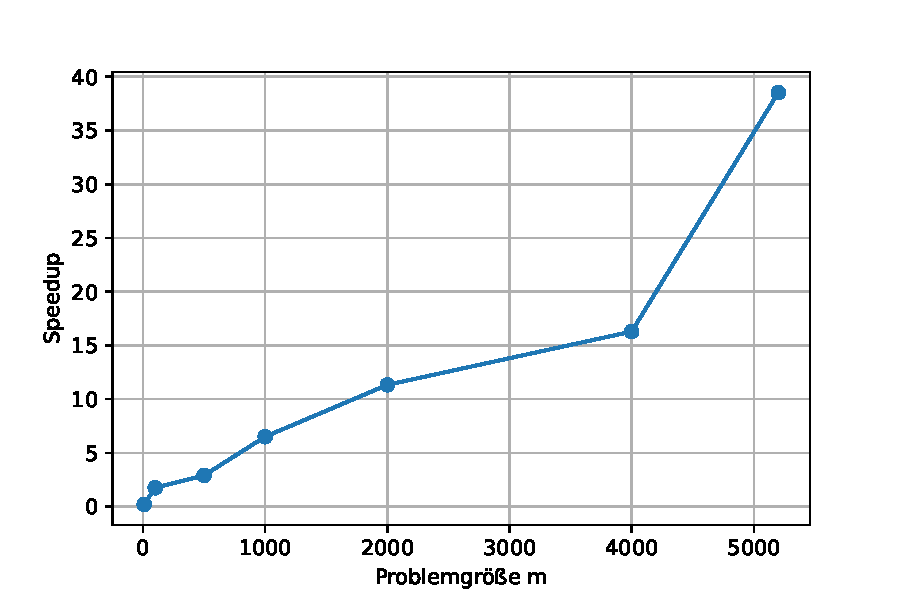
\includegraphics[width=9.2cm]{auto_speedup.pdf}}
	\caption{Matrix-Vektor-Multiplikation mit von \textit{OpenCL} automatisch festgelegter \code{local\_work\_size}.}
	\label{auto_lws}
\end{figure}
In Abb.~\ref{auto_lws} sind die Rechenzeit und der Speedup für die unterschiedlichen $m$ und eine von \textit{OpenCL} festgelegte \code{local\_work\_size} dargestellt. Es ist zu erkennen, dass die parallele Matrix-Vektor-Multiplikation insbesondere für sehr große $m$ mit wesentlich geringerem Zeitaufwand durchgeführt wird, als im sequentiellen Fall. Somit wird im Falle $m = 15000$ bereits ein Speedup $S_p \approx 75$ erreicht. Dies ist darauf zurückzuführen, dass jede Zeile der Matrix $\mathbf{A}$ als eigenes \textit{Work-Item} behandelt wird und somit mehrere Zeilen gleichzeitig abgewickelt werden können. Lediglich für sehr kleine $m$, wie in diesem Falle $m = 10$ wird das sequentielle Programm schneller ausgeführt, da der Overhead die ansonsten vorliegende Zeiteinsparung überwiegt. Auffällig ist, dass es einen Ausreißer für $m=1000$ gibt und die durch Streams parallelisierte Berechnung nur minimal schneller durchgeführt werden konnte als im sequentiellen Fall. Dies ist möglicherweise auf die allgemeine CPU-Auslastung zurückzuführen und bedarf nochmals einigen Untersuchungen. Da die CPU-Parallelisierung jedoch nicht Gegenstand der Aufgabenstellung ist, haben wir in diesem Fall zunächst darauf verzichtet.

Nun wurde die Anzahl der Work-Groups durch Variation der \code{local\_work\_size} $\in \{ 5, 10, 20, 25, 50, 100 \}$ verändert. Belässt man die Problemgröße konstant, z.B. $m = 10000$, zeigt sich in Abb.~\ref{lws_variation}a, dass nicht automatisch besonders viele oder besonders wenige Work-Groups die besten Ergebnisse liefern. So ist in unserem Beispiel \code{local\_work\_size = 20} eine besonders gute Wahl. Hier wurde im Vergleich zur zuvor durchgeführten Berechnung mit automatisch gewählter \textit{local size} sogar nochmals etwas Zeit eingespart. Zu einem ähnlichen Ergebnis kommt man bei Betrachtung von Abb.~\ref{lws_variation}b. Es ist bspw. erkennbar, dass sich die Rechenzeit für $m = 4000$ mit steigender \code{local\_work\_size} vergößert. Selbiges gilt auch für $m = 8000$. Um eine noch fundiertere Aussage treffen zu können, sollte man die \textit{local size} sowie die Problemgröße allerdings nochmals etwas kleinschrittiger variieren.
\begin{figure}[h!tb]
	\centering
	\subfigure[Ergebnisse für $m = 10000$.]{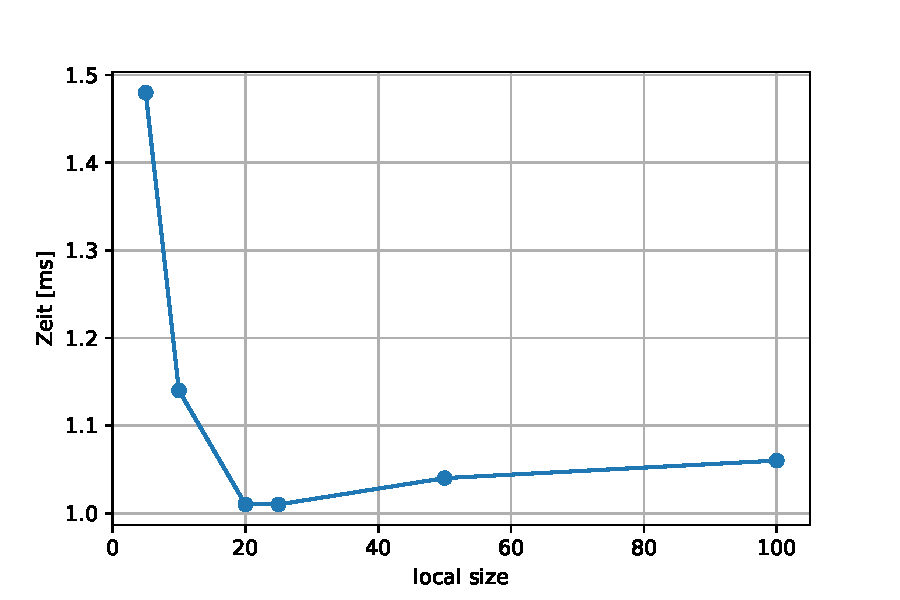
\includegraphics[width=9.2cm]{lws_variation.pdf}}\hspace{-1cm}
	\subfigure[Rechenzeit in ms.]{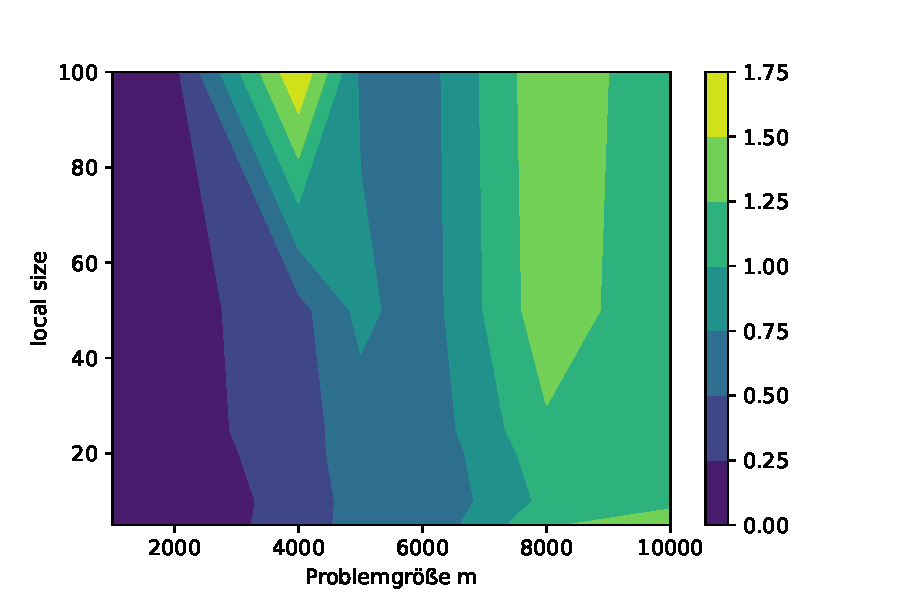
\includegraphics[width=9.2cm]{contour.pdf}}
	\caption{Variation der \code{local\_work\_size} und somit auch der Anzahl der Work-Groups.}
	\label{lws_variation}
\end{figure}


\chapter{Fazit}

In dieser Übung wurde eine Matrix-Vektor-Multiplikation in Form eines klassischen, sequentiellen Algorithmus als auch eines durch \textit{OpenCL} parallelisierten Algorithmus implementiert und die Performance der beiden Ansätze untersucht und verglichen. Es konnte festgestellt werden, dass durch die parallele Berechnung auf der GPU eine erhebliche Laufzeiteinsparung, insbesondere für sehr große Matrizen erreicht werden konnte. Desweiteren wurde gezeigt, dass eine geeignete Anzahl von \textit{OpenCL}-Work-Groups nicht einfach naiv gewählt werden kann, sondern einer Voruntersuchung bedarf. Insgesamt kann jedoch mithilfe von \textit{OpenCL} paralleler Code geschrieben werden, welcher im Vergleich zu seinem sequentiellen Gegenstück bei ausreichend zur Verfügung stehender Rechenleistung weitaus performanter ist. Der Mehraufwand bzgl. der Implementierung lohnt sich also deutlich.

\end{document}
